\begin{center}
\Huge
Harmoniske svingninger og trigonometriske funktioner
\end{center}

\section*{Harmoniske svingninger}
\stepcounter{section}

De trigonometriske funktioner $\cos(x)$ og $\sin(x)$ er periodiske funktioner, da 
\begin{align*}
\cos(x + 2\pi k) = \cos(x) 
\end{align*}
for alle heltal $k\in \mathbb{Z}$ og tilsvarende
\begin{align*}
\sin(x + 2\pi k) = \sin(x)
\end{align*}
for alle heltal $k$. Vi kan plotte $\cos(x)$ og $\sin(x)$, hvilket kan ses af Fig. \ref{fig:trig}
\begin{figure}[H]
\centering
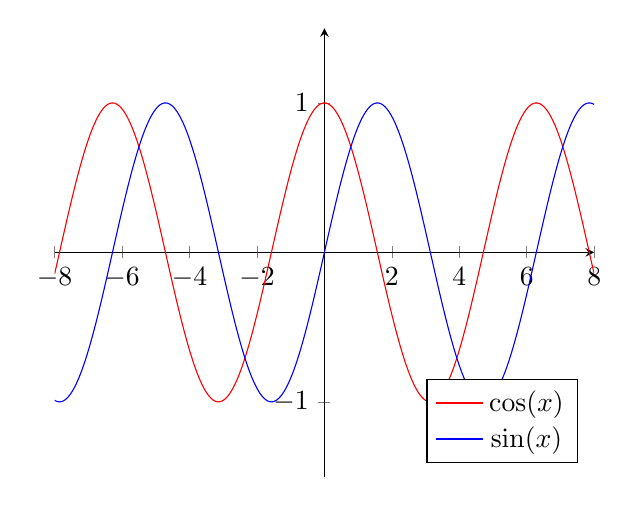
\begin{tikzpicture}
\begin{axis}[
axis lines = middle, 
xmin = -8, xmax = 8,
ymin = -1.5, ymax = 1.5,
legend pos = south east
]
\addplot[samples = 1000, color = red, domain = -8:8] {cos(deg(x))};
\addplot[samples = 1000, color = blue, domain = -8:8] {sin(deg(x))};
\legend{$\cos(x)$, $\sin(x)$}
\end{axis}
\end{tikzpicture}
\caption{Grafer for $\cos(x)$ og $\sin(x)$.}
\caption{fig:trig}
\end{figure}
Vi kan bruge trigonometriske funktioner til at modellere mange virkelige fænomener, da de er periodiske i natur. Vi kan eksempelvis bruge trigonometriske funktioner til at beskrive lyd og billedsignaler.

Da alle virkelige fænomener ikke har en periode på $2\pi$, så vil vi gerne kunne forkorte eller forlænge perioden. Vi vil også gerne kunne forskyde perioden, og vi vil gerne kunne øge \textit{amplituden}, så funktionen ikke kun går fra -1 til 1, men kan gå mellem større værdier. Desuden gælder der, at $\cos(x) = \sin(x + \frac{\pi}{2})$, så vi kan altid bruge $\sin$ til at beskrive $\cos$ og vice versa. Derfor giver vi følgende definition:
\begin{defn}[Harmoniske svingninger]
En sammenhæng 
\begin{align*}
y = A\cdot \sin(\omega t + \varphi)
\end{align*}
kaldes for en harmonisk svingning som funktion af tiden $t$. Konstanten $\omega$ kaldes for vinkelhastigheden, konstanten $\varphi$ kaldes for begyndelsesfasen og konstanten $A$ kaldes for amplituden. 
\end{defn}

\section*{Opgave 1}
I Geogebra tegn så funktionen 
\begin{align*}
y = A\sin(\omega x + \varphi).
\end{align*}
\begin{enumerate}[label=\roman*)]
\item Hvordan ændrer det på grafen for sammenhængen at ændre på $\varphi$?
\item Hvordan ændrer det på grafen at ændre på $\omega$?
\item Hvordan ændrer det på grafen at ændre på $A$?
\end{enumerate}

\section*{Opgave 2}
I Geogebra tegn så $\cos(x)$ og $\sin(x+k)$, og bestem $k$, så graferne er sammenfaldende. Argumentér ved brug af enhedscirklen for, at graferne er sammenfaldende i dette tilfælde. 

\section*{Opgave 3}
Vi kan ved en bestemt havn modellere vandstanden med den harmoniske svingning
\begin{align*}
f(t) = 1.2\sin(0.524t) + 3.4,
\end{align*}
hvor $t$ er tiden målt i timer og $f(t)$ er vandstanden i meter. 
\begin{enumerate}[label=\roman*)]
\item Tegn grafen for $f$ i Geogebra. 
\item På hvor mange timer er en periode? (Antallet af timer, før vandstanden er det samme igen)
\item Hvornår er vandstanden højest? Hvad med lavest?
\end{enumerate}
\section*{Opgave 4}
For den harmoniske svingning 
\begin{align*}
y = A\sin(\omega t + \varphi)
\end{align*}
kaldes længden på en periode $T$, så $y(t) = y(t+T)$ for svingningstiden, og antallet af perioder per tidsenhed $f$ kaldes for frekvensen. 
\begin{enumerate}[label=\roman*)]
\item Bestem et udtryk for svingningstiden $T$ for $y(t)$.
\item Bestem et udtryk for frekvensen $f$ for $y(t)$.
\end{enumerate}

\section*{Opgave 5}
En simpel model for lydbølger er en enkelt harmonisk svinging
\begin{align*}
P(t) = A\sin(2\pi f t),
\end{align*}
hvor $f$ er frekvensen målt i svingninger pr sekund (Hz), tid $t$ i sekunder, amplitude $A$ og $P(t)$ er tryk målt i decibel. 
\begin{enumerate}[label=\roman*)]
\item Kammertonen er 440 Hz. Plot i geogebra en harmonisk svingning med amplitude 70 og frekvens 440 Hz. Hvad er svingningstiden i dette tilfælde?
\item At gå en oktav op tilsvarer en fordobling af frekvensen, og at gå en oktav ned tilsvarer en halvering af frekvensen. Kammertonen er enstreget a: $a^1$. Vi betegner andre oktaver af a med
\begin{center}
\begin{tabular}{c|c|c|c|c|c|c|c|c}
Oktav & $A_2$ & $A_1$ & $A$ & $a$ & $a^1$ & $a^2$ & $a^3$ & $a^4$ \\
\hline
Frekvens&&&&&$440$Hz&&&
\end{tabular}
\end{center}
hvor $A_2$ her er laveste oktav og $a^4$ her er højeste. Udfyld resten af skemaet. 
\item Tegn grafen for den harmoniske svingning en tone over kammertonen og en tone under kammertonen. 
\end{enumerate}

